\documentclass[dvips,12pt]{article}

% Any percent sign marks a comment to the end of the line

% Every latex document starts with a documentclass declaration like this
% The option dvips allows for graphics, 12pt is the font size, and article
%   is the style

\usepackage[pdftex]{graphicx}
\usepackage{url}
\usepackage{lipsum}
\usepackage{placeins}
% These are additional packages for "pdflatex", graphics, and to include
% hyperlinks inside a document.

\setlength{\oddsidemargin}{0.25in}
\setlength{\textwidth}{6.5in}
\setlength{\topmargin}{-0.5in}
\setlength{\textheight}{8.5in}

% These force using more of the margins that is the default style

\begin{document}
\vspace{-4in}
% Everything after this becomes content
% Replace the text between curly brackets with your own

\title{EECS 341 Project Proposal: Bar Database}
\author{Dominique Owens, Daniel Grigsby, Lee Kelvin, Dina Benayad-Cherif}
\date{\today}

% You can leave out "date" and it will be added automatically for today
% You can change the "\today" date to any text you like


\maketitle

% This command causes the title to be created in the document

\section{Application Background}

% An article style is separated into sections and subsections with 
%   markup such as this.  Use \section*{Principles} for unnumbered sections.

Our project describes and implements a functioning bar. Through this database, the profits, employees, regular customers and menus of a bar could be managed. Cash registers would be able to insert purchases of food into the database, and managers could add and remove employees, change wages and run the restaurant. 


\section{Data Description}
We will keep track of the following statistics for each entity in the database.
\begin{enumerate}

\item Employees
\begin{enumerate}
\item Name
\item Salary 
\item Date hired 
\item Bills served 
\item Customers served
 \item Other Employees Managed
\end{enumerate}


\item Customers
\begin{enumerate}
\item Name
 \item Items purchased 
 \item Money spent
\item Age
\end{enumerate}

\item Drinks
\begin{enumerate}
\item Name
 \item price 
\item quantity sold
\item Is alcoholic or not
\end{enumerate}

\item Food
\begin{enumerate}
\item Name
 \item price
 \item quantity sold
\item Gluten free, vegan or neither
\end{enumerate}

\item Bills / Receipts
\begin{enumerate}
\item Total price
\item Items on bill
\item Customer that made the purchase
\item Employee that waited on the customer
\item Tip given by customer
\end{enumerate}

\end{enumerate}
\section{Schema}
\noindent
Customer(\underline{cid}, name, age) \\
\noindent
FoodPurchase(\underline{cid}, \underline{fid}, qty) \\ \begin{enumerate}
\item cid in FoodPurchase is a foreign key referencing cid in Customer
\item fid in FoodPurchase is a foreign key referencing fid in FoodItem
\end{enumerate}
\noindent
DrinkPurchase(\underline{cid}, \underline{did}, qty) \\ \begin{enumerate}
\item cid in DrinkPurchase is a foreign key referencing cid in Customer
\item did in DrinkPurchase is a foreign key referencing did in Drink
\end{enumerate}
\noindent
FoodItem(\underline{fid}, name, pid, vegan, gluten-free) \\ \begin{enumerate}
\item pid is a foreign key referencing pid in Pricetable \end{enumerate}
\noindent
Drink(\underline{did}, name, pid, alcoholic) \begin{enumerate}
\item pid is a foreign key referencing pid in Pricetable \end{enumerate}
\noindent
Pricetable(\underline{pid}, price) \\

\noindent
Bill(\underline{billNo}, \underline{cid}, \underline{eid}, totalprice, tip) \\  \begin{enumerate}
\item cid is a foreign key referencing cid in Customer
\item eid is a foreign key referencing eid in Employee 
\end{enumerate} 
\noindent
Employee(\underline{eid}, salary, name, date-hired) \\


\noindent
Manager(\underline{mid}, name, eid) \\ \begin{enumerate}
\item eid is a foreign key referencing eid in Employee
\end{enumerate} 

 






\FloatBarrier
\section{ER Diagram}
\begin{figure}
  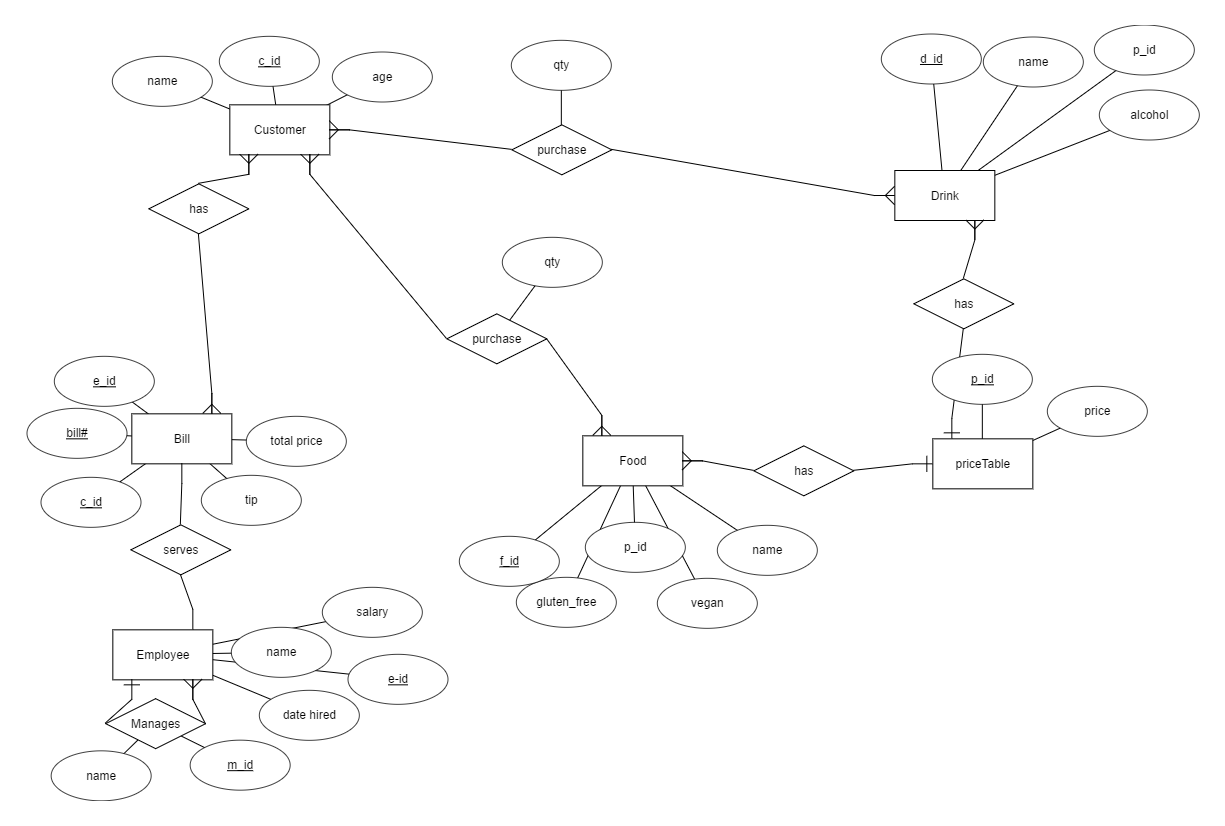
\includegraphics[width=\linewidth]{er.png}
  \caption{ER Diagram.}
  \label{fig:er1}
\end{figure}
\FloatBarrier



\end{document}
